\section{Квазигруппы и правильные семейства}
\begin{frame}[plain, noframenumbering]
    \begin{center}
        \Huge
        Квазигруппы и правильные семейства
    \end{center}
\end{frame}

\subsection{Квазигруппы}

\begin{frame}
    \frametitle{Квазигруппы: определение}
    \begin{dfn}
        Квазигруппа~---~множество $Q$ с операцией ${\circ \colon Q \times Q \to Q}$ со свойством: $\forall \; a, b \in Q \quad \exists ! x, y \in Q:$
        \[
            a \circ x = b, y \circ a = b.
        \]
    \end{dfn}

    \pause
    Операции левого и правого умножения задают перестановки:
    \[ 
        L_a \colon Q \to Q,\quad L_a(x) = a \circ x 
    \]
    \[
        R_a \colon Q \to Q,\quad R_a(y) = y \circ a 
    \]
    \[
        L_a, R_a \in S_Q
    \]
\end{frame}


\begin{frame}
    \frametitle{Алгебраические свойства квазигрупп}
    % С точки зрения криптографических приложений наиболее интересны следующие свойства
    \begin{itemize}
        \item Количество ассоциативных троек в квазигруппе
        \item Полиномиальная полнота квазигруппы
        \item Наличие подквазигрупп
    \end{itemize}
\end{frame}


\begin{frame}
    \frametitle{Свойства квазигрупп: ассоциативность}
    \begin{dfn}
        Ассоциативная тройка~---~$a, b, c \in Q:$
        \[
            (a \circ b) \circ c = a \circ (b \circ c).
        \]

        Индекс ассоциативности квазигруппы $Q$~---~число ассоциативных троек в $Q$.
    \end{dfn}
\end{frame}



\begin{frame}
    \frametitle{Свойства квазигрупп: полиномиальная полнота}
    \begin{dfn}
        $Q$ полиномиально полна, если любую $n$-арную функцию $Q^n \to Q$ можно выразить через операцию умножения $\circ$ в квазигруппе и подстановку констант.

        \pause
        Более формально: замыкание операции $\circ$ и всех нуль-арных функций (констант) порождает все множество функций на $Q:$
        \[
            [\circ \cup \{a_1, \ldots, a_n\}] = \mathcal{O}(Q).
        \]
    \end{dfn}
\end{frame}


\subsection{Правильные семейства}

\begin{frame}
    \frametitle{Правильные семейства булевых функций}
    \begin{dfn}
        Семейство булевых функций 
        \[ 
            F = (f_1(x_1, \ldots, x_n), \ldots, f_n(x_1, \ldots, x_n))
        \]
        называется правильным, если для любых двух неравных двоичных наборов 
        \[
            \alpha = (\alpha_1, \ldots, \alpha_n), \quad 
            \beta = (\beta_1, \ldots, \beta_n), \quad 
            \alpha \ne \beta,
        \]
        выполняется следующее условие:
        \pause
        \[ 
            \exists i: 
            \alpha_i \ne \beta_i, \quad f_i(\alpha) = f_i(\beta). 
        \]
        Число $n$ будем называть размером правильного семейства.
    \end{dfn}
\end{frame}

\subsection{Построение квазигрупп по правильному семейству}

\begin{frame}
    \frametitle{<<Внутренняя>> конструкция}
    \begin{thm}
        Пусть 
        \[
            x, y \in \mathbb{Z}_2^n, (f_1, \ldots f_n) - \text{семейство булевых функций.}
        \]
        Рассмотрим следующую операцию на множестве $\mathbb{Z}_2^n:$
        \[
            x \circ y = x \oplus y \oplus f^{\; \pi}(x, y),
        \]
        \pause
        где за $f^{\; \pi}(x, y)$ обозначена следующая конструкция:
        \[
            f^{\; \pi}(x, y) = 
            (f_1(\pi_1(x_1, y_1), \ldots, \pi_n(x_n, y_n)), 
            \ldots, f_n(\pi_1(x_1, y_1), \ldots \pi_n(x_n, y_n))),
        \]
        \[
            \pi_i : \mathbb{Z}_2^2 \to \mathbb{Z}_2 - \text{произвольные булевы функции.}
        \]
        \pause
        Тогда операция $\circ : \mathbb{Z}_2^n \times \mathbb{Z}_2^n \to \mathbb{Z}_2^n$ задает структуру квазигруппы на $\mathbb{Z}_2^n$ для любых функций $\pi_i$ тогда и только тогда, когда $(f_1, \ldots, f_n)$~---~правильное семейство.
    \end{thm}
\end{frame}


\begin{frame}
    \frametitle{<<Внешняя>> конструкция}
    \begin{thm}
        Cемейство $F(x_1, \ldots, x_n)$ является правильным тогда и только тогда, когда для любого набора отображений $\psi$ вида: 
        \[
            \psi = (\psi_1, \ldots, \psi_n)^T,
            \quad
            \psi_i : \{0, 1\} \to \{0, 1\},
        \]
        отображение
        \[ 
            x \oplus \psi(F(x)) = 
            \begin{bmatrix}
                x_1 \oplus \psi_1(f_1(x_1, \ldots, x_n))\\
                \vdots \\
                x_n \oplus \psi_n(f_n(x_1, \ldots, x_n))
            \end{bmatrix}
        \]
        является биекцией $\{0, 1\}^n \to \{0, 1\}^n.$
        \pause
        В таком случае 
        \[
            x \ast y = x \oplus \phi(F(x)) \oplus y \oplus \psi(G(y)),
        \]
        задает структуру квазигруппы на $Q = \mathbb{Z}_2^n$ ($F, G$~---~правильные).
    \end{thm}
\end{frame}


\begin{frame}
    \frametitle{Возможные обобщения}
    \begin{itemize}
        \item Понятие правильности обобщается на любые системы множеств
        \pause
        \item С помощью правильных семейств можно задавать классы квазигрупп над произвольными абелевыми группами (и более общо~---~над прямым произведением 3-квазигрупп)
        \pause
        \item Также можно задавать <<многомерные>> латинские квадраты (гиперкубы)
    \end{itemize}
\end{frame}


\begin{frame}
    \frametitle{Проверка алгебраических свойств}
    \begin{itemize}
        \item Проверка полиномиальной полноты, наличия подквазигрупп и вычисление индекса ассоциативности может быть произведено за полиномиальное время от размера латинского квадрата (экспоненциальное по размеру правильного семейства).
        \pause
        \item Экспериментальные результаты по полиномиальной полноте и индексу ассоциативности для квазигрупп, порожденных правильными семействами малых размеров.
    \end{itemize}
\end{frame}





\section{Свойства правильных семейств}
\begin{frame}[plain, noframenumbering]
    \begin{center}
        \Huge
        Свойства правильных семейств булевых функций
    \end{center}
\end{frame}

\subsection{Преобразования, сохраняющие правильность}

\begin{frame}
    \frametitle{Сохранение правильности при перестановках}
    \begin{thm}
        Пусть $\sigma \in S_n,$ и $F(x_1, \ldots, x_n)$~---~правильное семейство.
        Рассмотрим семейство $\sigma(F),$ которое получено одновременной перестановкой индексов переменных и индексов входящих в семейство функций:
        \[
            f_i(x_1, \ldots, x_n) \to 
            f_{\sigma(i)}(x_{\sigma(1)}, \ldots, x_{\sigma(n)}).
        \]
        Семейство $\sigma(F)$ также является правильным.
    \end{thm}
\end{frame}


\begin{frame}
    \frametitle{Сохранение правильности при сдвигах}
    \begin{thm}
        Пусть $A = (a_1, \ldots, a_n) \in \{0, 1\}^n.$
        Рассмотрим семейство $G(x) = F(x) \oplus A:$
        \[
            G(x) = F(x) \oplus A = 
            \begin{bmatrix}
                f_1(x_1, \ldots, x_n) \oplus a_1 \\
                \vdots \\
                f_n(x_1, \ldots, x_n) \oplus a_n \\
            \end{bmatrix}.
        \]
        $F(x)$ правильное тогда и только тогда,
        когда $G(x) = F(x) \oplus A$ является правильным.
    \end{thm}
\end{frame}


\begin{frame}
    \frametitle{Сохранение правильности при проекциях}
    \begin{thm}
        Пусть $F$~---~правильное семейство булевых функций размера $n,$ зафиксируем $i \in \{1, \ldots, n\}$ и константу ${a \in \{0, 1\}.}$
        Тогда семейство $G,$ полученное из $F$ подстановкой вместо $x_i$ константы $a$ и вычеркиванием функции $f_i$ является правильным семейством размера $(n-1)$:
        \[
            G(x_1,\ldots,x_{i-1}, x_{i+1}, \ldots, x_n) = 
            \begin{bmatrix}
                f_1(x_1,\ldots,x_{i-1}, a, x_{i+1}, \ldots, x_n) \\
                \vdots \\
                f_{i-1}(x_1,\ldots,x_{i-1}, a, x_{i+1}, \ldots, x_n) \\
                f_{i+1}(x_1,\ldots,x_{i-1}, a, x_{i+1}, \ldots, x_n) \\
                \vdots \\
                f_{n}(x_1,\ldots,x_{i-1}, a, x_{i+1}, \ldots, x_n) \\
            \end{bmatrix}.
        \]
    \end{thm}
\end{frame}


\begin{frame}
    \frametitle{Выделенный класс правильных семейств}
    Используя свойства сохранения правильности при различных преобразованиях, было доказано, что все семейства вида
    \begin{equation}
        \begin{bmatrix}
            0 \\
            x_1 \\
            x_1 \oplus x_2 \\
            \vdots \\
            x_1 \oplus x_2 \oplus \ldots \oplus x_{n-1}
            \end{bmatrix}
            \bigoplus
            \begin{bmatrix}
            \bigoplus_{i < j, \; i, j \ne 1}^n \; x_i x_j \\
            \bigoplus_{i < j, \; i, j \ne 2}^n \; x_i x_j \\
            \bigoplus_{i < j, \; i, j \ne 3}^n \; x_i x_j \\
            \vdots \\
            \bigoplus_{i < j, \; i, j \ne n}^n \; x_i x_j \\
        \end{bmatrix}
    \end{equation}
    являются правильными.
\end{frame}


\subsection{Свойства правильных семейств как отображений}

\begin{frame}
    \frametitle{Количество прообразов}
    \begin{thm}
        Пусть $F = (f_1, \ldots, f_n)$~---~правильное семейство булевых функций.
        Тогда для любого $A \in \{0, 1\}^n$ число решений уравнения
        \(
            F(x) = A
        \)
        всегда четно.
    \end{thm}
    \pause
    \begin{cor}
        У перестановки $x \to x \oplus \phi(F(x))$ всегда четное число неподвижных точек.
    \end{cor}
\end{frame}


\begin{frame}
    \frametitle{Неподвижные точки}
    \begin{thm}
        У отображения $x \to F(x)$, где $F$~---~правильное семейство булевых функций, всегда существует единственная неподвижная точка.
    \end{thm}
    \pause
    \begin{thm}
        Семейство $F$ является правильным семейством булевых функций тогда и только тогда, когда у отображения $x \to F(x)$ и у всевозможных ограничений отображения на подкубы булева куба существует единственная неподвижная точка.
    \end{thm}
\end{frame}


\begin{frame}
    \frametitle{Геометрическая интерпретация правильного семейства}
    \begin{thm}
        Существует взаимно-однозначное соответствие между правильными семействами булевых функций $F$ и ориентациями с единственным стоком на графах булевых кубов $\mathbb{E}_n$
    \end{thm}

    \centering
    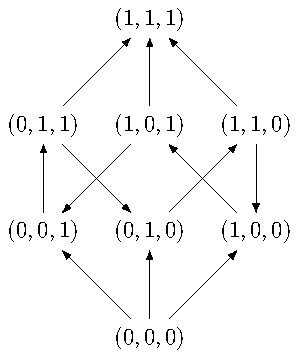
\includegraphics[width=0.25\linewidth]{fig1}
\end{frame}


\begin{frame}
    \frametitle{Следствия геометрической интерпретации}
    \begin{cor}
        Пусть семейство булевых функций задано в виде конъюнктивной нормальной формы.
        Тогда задача распознавания правильности семейства является $coNP$"=полной.
    \end{cor}
    \pause
    \begin{cor}
        Обозначим за $T(n)$ количество правильных семейств размера $n.$ 
        Тогда $T(n) \ge 4 (T(n-1))^2 $ 
    \end{cor}
\end{frame}


\begin{frame}
    \frametitle{Следствия геометрической интерпретации}
    \begin{itemize}
        \item Нижние и верхние границы на число правильных семейств размера $n.$
        \item Показано, что число семейств специального вида (т.н. треугольные семейства) составляют экспоненциально малую часть от всех правильных семейств булевых функций.
    \end{itemize}
\end{frame}


\section{Применение квазигрупп в криптографии}
\begin{frame}[plain, noframenumbering]
    \begin{center}
        \Huge
        Применение квазигрупп в криптографии
    \end{center}
\end{frame}


\begin{frame}
    \begin{itemize}
        \item Односторонние и хэш-функции (легко вычислить, трудно обратить)
        \item Поточные шифры (<<посимвольная>> обработка потока)
        \item Протоколы асимметричной криптографии: согласование ключа, шифрование, гомоморфное шифрование (луповые кольца)
        \item Предложено использовать квазигруппы в качестве платформы для задания шифрования, сохраняющего формат (формат шифртекста совпадает с форматом исходного текста)
    \end{itemize}
\end{frame}
